\documentclass[12pt,a4paper]{article}

\usepackage[utf8]{inputenc}
\usepackage[T1]{fontenc}
\usepackage{graphicx}
\usepackage{amsmath}
\usepackage[margin=2.5cm]{geometry}
\usepackage{float}
\usepackage{tikz}
\usepackage{pgfplots}
\pgfplotsset{compat=1.16}

\title{Measurement of Ohmic Resistances, Bridge Circuits
and Internal Resistances of Voltage Sources}

\author{
Terje\\
\texttt{terje.frisse@uni-oldenburg.de}\\
Ayoub\\
\texttt{ayoub.jaziri@uni-oldenburg.de}\\
Group 7
}

\date{\today}

\begin{document}

\maketitle
\section{Experiments}
\subsection{Wheatstone Bridge}
In this part, we measured an unknown resistance $R$ with a Wheatstone bridge. This method does not depend on the quality of the current and voltage meters.

\subsubsection{Method}
The bridge was built as in Fig.~4 of the script [1]. A constantan wire of length $l = l_1 + l_2 = 1.000$~m was connected to the unknown resistor $R$ and to a resistor decade as comparison resistor $R_3$. We chose $R_3 = 1.2$~k$\Omega$, which is close to $R$, so that $l_1 \approx l_2$ and the error is small. A voltage supply was used as source. The sliding contact was moved along the wire until the ammeter between the two branches showed no current. The bridge is balanced then, and the lengths $l_1$ and $l_2$ were read from the scale with a reading error of 0.5~mm. The resistance follows from
\begin{equation}
  R = R_3 \,\frac{l_2}{l_1}.
\end{equation}

\subsubsection{Results and Discussion}
The measured values are listed in Tab.~\ref{tab:wheat}. With them we get
\begin{equation}
  R = (1190 \pm 14)~\Omega.
\end{equation}
The maximum error was calculated with
\begin{equation}
  \frac{\Delta R}{R} = \frac{\Delta R_3}{R_3} + \frac{\Delta l_1}{l_1} + \frac{\Delta l_2}{l_2}.
\end{equation}
It is dominated by the 1\% error of the decade, since the length errors contribute only about 0.2\%.

\begin{table}[H]
  \centering
  \caption{Measured values of the balanced Wheatstone bridge and the resulting resistance.}
  \label{tab:wheat}
  \begin{tabular}{cccc}
    \hline
    $R_3$ / $\Omega$ & $l_1$ / mm & $l_2$ / mm & $R$ / $\Omega$ \\
    \hline
    $1200 \pm 12$ & $502.0 \pm 0.5$ & $498.0 \pm 0.5$ & $1190 \pm 14$ \\
    \hline
  \end{tabular}
\end{table}
\subsection{Specific Resistance of Tap Water}
In this experiment, we wanted to find the specific resistance $\rho_w$ of tap water from the resistance between two copper plates.

\subsubsection{Method}
Two parallel copper plates of width $b = [\ldots]$~m were placed at a distance $l = [\ldots]$~m in a water basin with tap water. The plates have a thickness of $(1.5 \pm 0.05)$~mm. By lifting the basin, the immersion depth $d$ of the plates was changed. To avoid polarization effects, we used a sinusoidal alternating voltage without dc offset from the FG, and both multimeters (Agilent) were set to ac mode. For each depth, the voltage $U$ and the current $I$ were measured (circuit A of the script [1]). The resistance of the water between the plates is
\begin{equation}
  R_w = \rho_w \,\frac{l}{b}\,\frac{1}{d},
\end{equation}
so $\rho_w$ follows from the slope $m = \rho_w\, l/b$ of $R_w$ plotted against $1/d$.

\subsubsection{Results and Discussion}
The values are listed in Tab.~\ref{tab:water} and shown in Fig.~\ref{fig:water}. A linear fit gives a slope of $m = (0.18 \pm 0.19)$~k$\Omega$\,m, which is consistent with zero.

\begin{table}[H]
  \centering
  \caption{Voltage $U$, current $I$ and resulting resistance $R_w = U/I$ for different immersion depths $d$.}
  \label{tab:water}
  \begin{tabular}{cccc}
    \hline
    $d$ / mm & $U$ / V & $I$ / mA & $R_w$ / k$\Omega$ \\
    \hline
    10 & 2.158 & 0.018 & 120 \\
    20 & 2.0   & 0.023 & 87.0 \\
    30 & 1.87  & 0.021 & 89.0 \\
    40 & 1.64  & 0.017 & 96.5 \\
    50 & 1.52  & 0.015 & 101 \\
    60 & 1.457 & 0.013 & 112 \\
    \hline
  \end{tabular}
\end{table}

\begin{figure}[H]
  \centering
  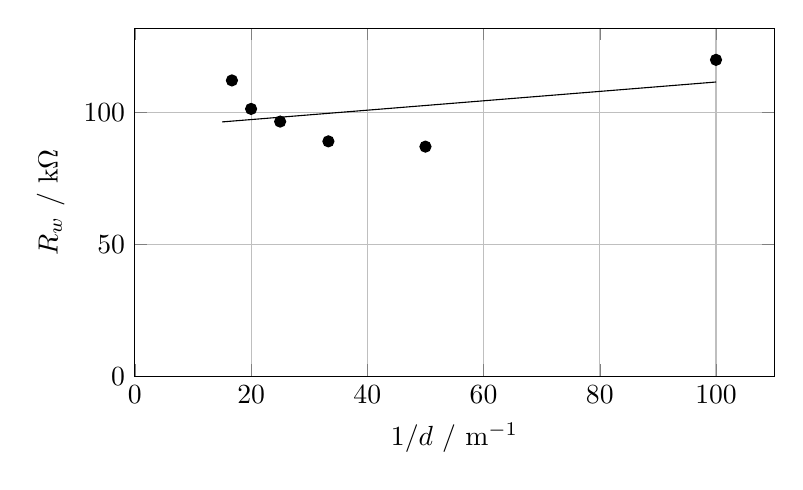
\begin{tikzpicture}
    \begin{axis}[width=0.8\textwidth, height=6cm, grid=major, xmin=0, ymin=0,
      xlabel={$1/d$ / m$^{-1}$}, ylabel={$R_w$ / k$\Omega$}]
      \addplot[only marks, mark=*] coordinates
        {(100,119.9)(50,87.0)(33.3,89.0)(25,96.5)(20,101.3)(16.7,112.1)};
      \addplot[no marks, domain=15:100] {93.7+0.178*x};
    \end{axis}
  \end{tikzpicture}
  \caption{Resistance $R_w$ of the water as a function of $1/d$ with linear fit.}
  \label{fig:water}
\end{figure}

We expected $R_w$ to fall with increasing $d$, so the points should lie on a line through the origin with positive slope. This was not the case: $R_w$ stays around 100~k$\Omega$ and even rises with $d$ for $d \geq 20$~mm. The fit therefore does not give a usable value of $\rho_w = m\,b/l$. The resistance is also much larger than expected for tap water, for which the script gives $\rho_w$ of about 10 to 20~$\Omega$m [1]. Possible reasons are an error in the current range, a change of the water level or the plate position during the series, and poor contact at small depths. Thus, $\rho_w$ could not be determined reliably, and the measurement should be repeated.
\end{document}